\documentclass[12pt,a4paper]{article}

\usepackage[T1,T2A]{fontenc}
\usepackage[utf8]{inputenc}
\usepackage[english, russian]{babel}
\usepackage{indentfirst}
\usepackage{misccorr}
\usepackage{graphicx}
\usepackage{amsmath}
\usepackage{graphicx}
\usepackage{float}
\usepackage[left=20mm,right=10mm, top=20mm,bottom=20mm,bindingoffset=0mm]{geometry}

\setlength{\parskip}{6pt}\graphicspath{{images/}}\DeclareGraphicsExtensions{.png}

\begin{document}

    \begin{titlepage}
        \begin{center}
            \large
            Санкт-Петербургский политехнический университет\\Петра Великого\\
            \vspace{0.5cm}
            Институт прикладной математики и механики\\
            \vspace{0.25cm}
            Кафедра «Прикладная математика»
            \vfill
            \textsc{\LARGE\textbf{Отчет по лабораторной работе №3}}\\[5mm]
            \Large
            по дисциплине\\"Математическая статистика"
        \end{center}
        \vfill
        \begin{tabular}{l p{175pt} l}
            Выполнил студент \\ группы 3630102/80201 && Хрипунков Дмитрий Викторович
            \vspace{0.25cm}
            \\Проверил \\ доцент, к.ф.-м.н. && Баженов Александр Николаевич
        \end{tabular}
        \vfill
        \begin{center}
            Санкт-Петербург \\ 2021 г.
        \end{center}
    \end{titlepage}

\newpage
\begin{center}
    \tableofcontents
    \setcounter{page}{2}
\end{center}
\newpage
\begin{center}
    \listoffigures
\end{center}

\newpage
\section{Постановка задачи}
Для 5 распределений:
\begin{itemize}
    \item Нормальное распределение $N(x,0,1)$
    \item Распределение Коши $C(x,0,1)$
    \item Распределение Лапласа $L(x,0,\frac{1}{\sqrt{2}})$
    \item Распределение Пуассона $P(k,10)$
    \item Равномерное распределение $U(x,-\sqrt{3},\sqrt{3})$
\end{itemize}

Необходимо:
\begin{enumerate}
    \item Сгенерировать выборки размером 20 и 100 элементов
    \item Построить для них боксплот Тьюки 
    \item Для каждого распределения определить долю выбросов экспериментально (сгенерировав выборку, соответствующую распределению 1000раз, и вычислив среднюю долю выбросов) и сравнить с результатами, полученными теоретически
\end{enumerate}

\section{Теория}
\subsection{Рассматриваемые распределения}
Плотности:
\begin{itemize}
		\item Нормальное распределение
		    \begin{equation}
			    N(x,0,1)=\frac{1}{\sqrt{2\pi}}e^{-\frac{x^2}{2}}
			    \label{normal} 
			\end{equation}
		\item Распределение Коши
		    \begin{equation}
				C(x,0,1)=\frac{1}{\pi}\frac{1}{x^2+1}
				\label{cauchy}
			\end{equation} 
		\item Распределение Лапласа
		    \begin{equation}
				L(x,0,\frac{1}{\sqrt{2}})=\frac{1}{\sqrt{2}}e^{-\sqrt{2}|x|}
				\label{laplace} 
			\end{equation}
		\item Распределение Пуассона
		    \begin{equation}
				P(k,10)=\frac{10^k}{k!}e^{-10}
				\label{poisson}
			\end{equation}
		\item Равномерное распределение
		    \begin{equation}
				U(x,-\sqrt{3},\sqrt{3})=
				\begin{cases}
					\frac{1}{2\sqrt{3}},|x|\leq\sqrt{3}\\0,|x|>\sqrt{3}
				\end{cases}
				\label{uniform}
			\end{equation}
\end{itemize}

\subsection{Боксплот Тьюки}
\textit{Боксплот Тьюки} - график, использующийся в описательной статистике, компактно изображающий одномерное распределение вероятностей. С помощью такого графика можно в удобной форме показать множество характеристик распределения, как медиану, нижний и верхний квартили, минимальное и максимальное значение и выбросы.

\subsection{Построение}
При построении боксплота границами выступают первый и третий квартили, серединой ящика выступает медиана. Концы "усов" - края статистически значимой выборки (без выбросов). Длина определяется по формуле:
        \begin{equation}
            X_1 = Q_1 - \frac{3}{2}(Q_3 - Q_1), X_2 = Q_3 + \frac{3}{2}(Q_3 - Q_1)
        \label{eq:mustache}
        \end{equation}
$X_1$ — нижняя граница уса, $X_2$ — верхняя граница уса, $Q_1$ - первый квартиль, $Q_3$ - третий квартиль.

Выбросы выходят за границы усов и отображаются на графике в виде кружков

\subsection{Теоретическая вероятность выбросов}
Можно вычислить теоретически первый и третий квартили $Q_1^T$ и $Q_3^T$ и нижнюю и верхнюю границы уса $X_1^T$ и $X_2^T$ по формуле \eqref{eq:mustache}. После этого можно определить выбросы $x:$
\begin{equation}
	\left[
	\begin{array}{ll}
        x<X_1^T\\
		x>X_2^T\\
	\end{array}
    \right.
\end{equation}

Теоретическая вероятность выбросов:
\begin{itemize}
    \item для непрерывных распределений:
        \begin{equation}
		    P_B^T=P(x<X_1^T)+P(x>X_2^T)=F(X_1^T)+(1-F(X_2^T))
	    \end{equation}
	\item для дискретных распределений:
	    \begin{equation}
		    P_B^T=P(x<X_1^T)+P(x>x_2^T)=(F(X_1^T)-P(x=X_1^T))+(1-F(X_2^T))
	    \end{equation}
\end{itemize}
Где $F(X)=P(x\leq{X})$ - функция распределения

\section{Реализация}
Лабораторная работа выполнена на языке Python в виртуальной среде Anaconda с интерпретатором версии 3.9 в среде разработки Visual Studio Code. Дополнительные зависимости:
\begin{itemize}
    \item scipy
    \item numpy
    \item matplotlib
    \item seaborn
\end{itemize}

Исходный код размещён в git-репозитории на GitHub: \\ https://github.com/ThinkingFrog/MathStat

\section {Результаты}
\subsection{Графики}
\begin{figure}[H]
    \centering
    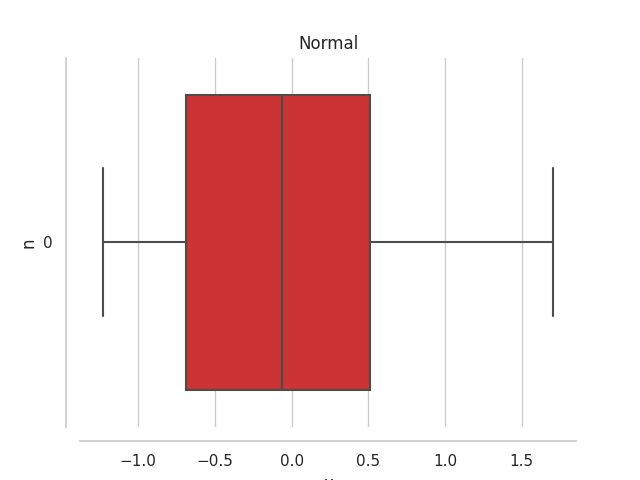
\includegraphics[scale=0.8]{Normal20.png}
    \caption{Нормальное распределение с размером выборки 20}
    \label{fig:normal}
\end{figure}

\begin{figure}[H]
    \centering
    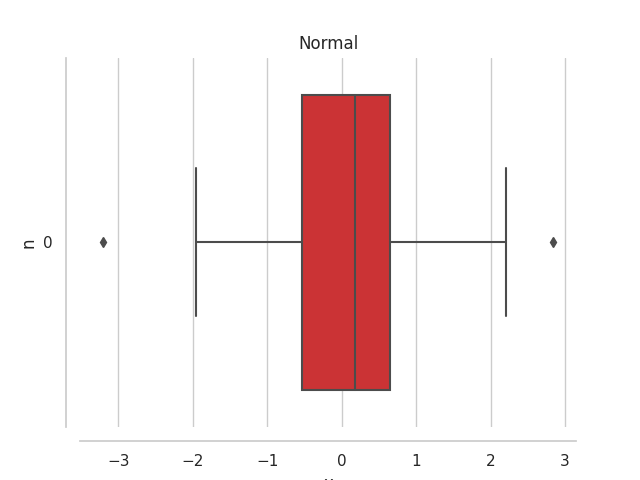
\includegraphics[scale=0.8]{Normal100.png}
    \caption{Нормальное распределение с размером выборки 100}
    \label{fig:normal}
\end{figure}

\begin{figure}[H]
    \centering
    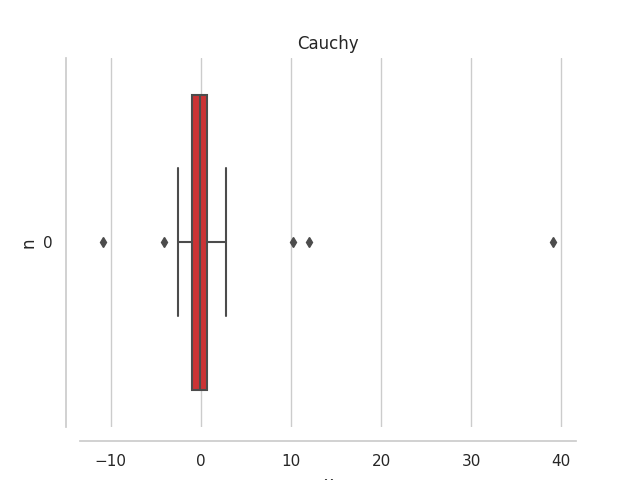
\includegraphics[scale=0.8]{Cauchy20.png}
    \caption{Распределение Коши с размером выборки 20}
    \label{fig:normal}
\end{figure}

\begin{figure}[H]
    \centering
    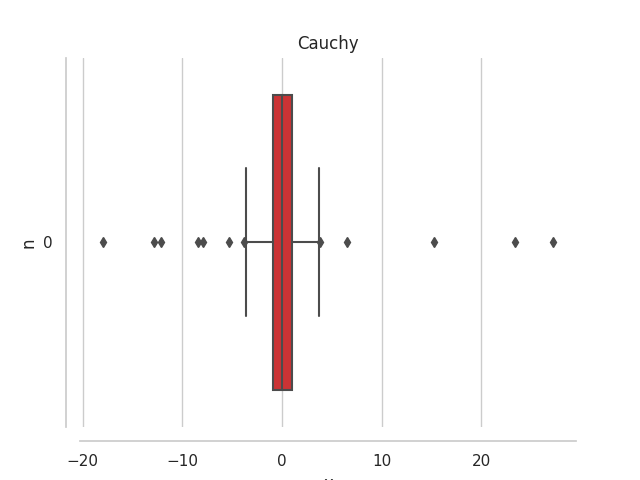
\includegraphics[scale=0.8]{Cauchy100.png}
    \caption{Распределение Коши с размером выборки 100}
    \label{fig:normal}
\end{figure}

\begin{figure}[H]
    \centering
    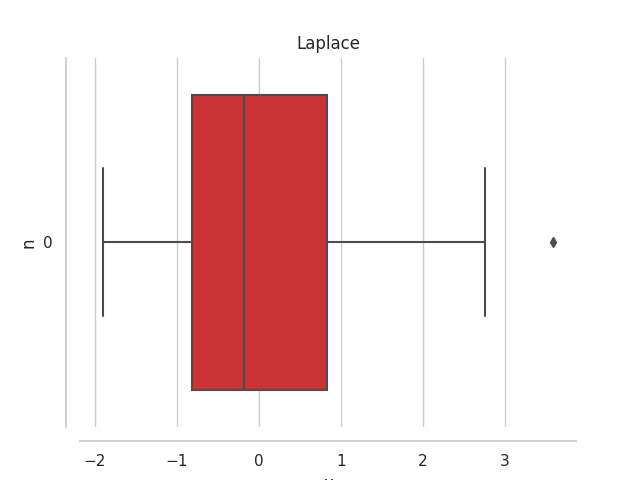
\includegraphics[scale=0.8]{Laplace20.png}
    \caption{Распределение Лапласа с размером выборки 20}
    \label{fig:normal}
\end{figure}

\begin{figure}[H]
    \centering
    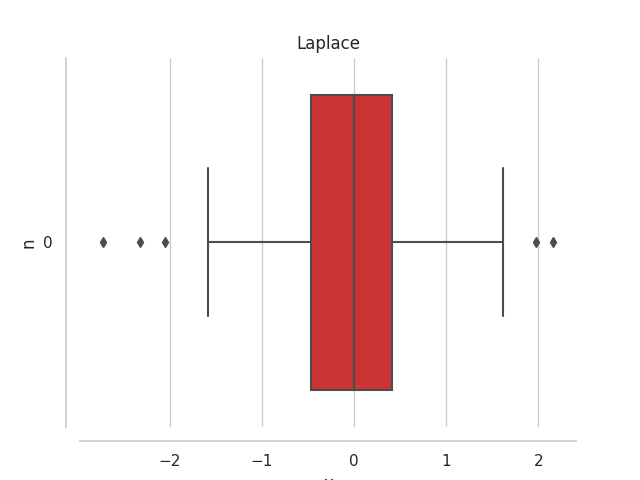
\includegraphics[scale=0.8]{Laplace100.png}
    \caption{Распределение Лапласа с размером выборки 100}
    \label{fig:normal}
\end{figure}

\begin{figure}[H]
    \centering
    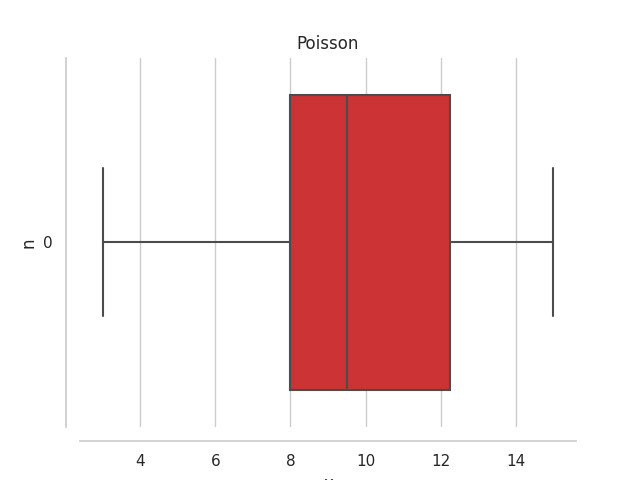
\includegraphics[scale=0.8]{Poisson20.png}
    \caption{распределение Пуассона с размером выборки 20}
    \label{fig:normal}
\end{figure}

\begin{figure}[H]
    \centering
    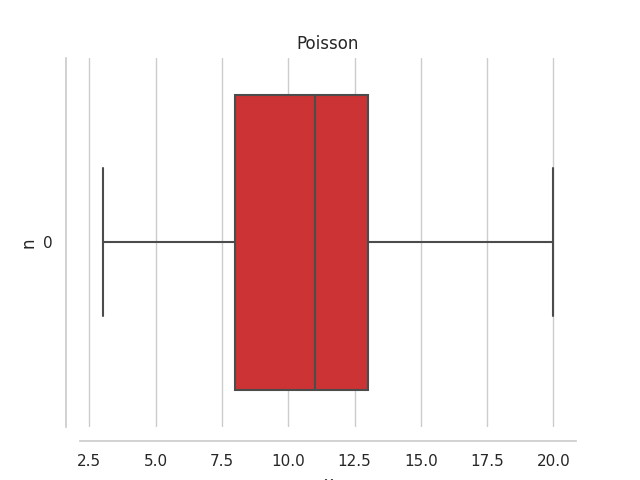
\includegraphics[scale=0.8]{Poisson100.png}
    \caption{Распределение Пуассона с размером выборки 100}
    \label{fig:normal}
\end{figure}

\begin{figure}[H]
    \centering
    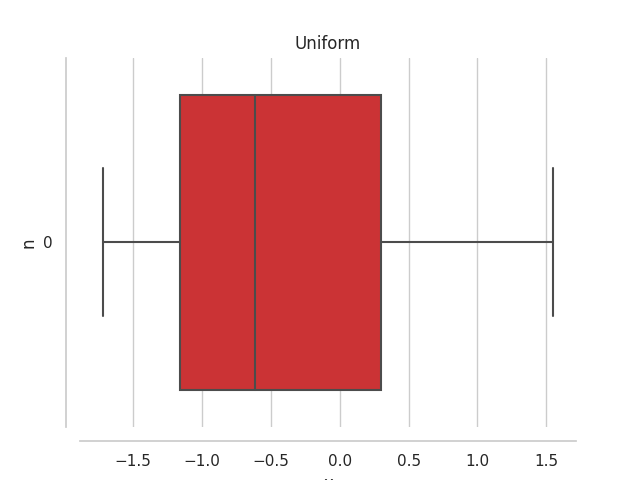
\includegraphics[scale=0.8]{Uniform20.png}
    \caption{Равномерное распределение с размером выборки 20}
    \label{fig:normal}
\end{figure}

\begin{figure}[H]
    \centering
    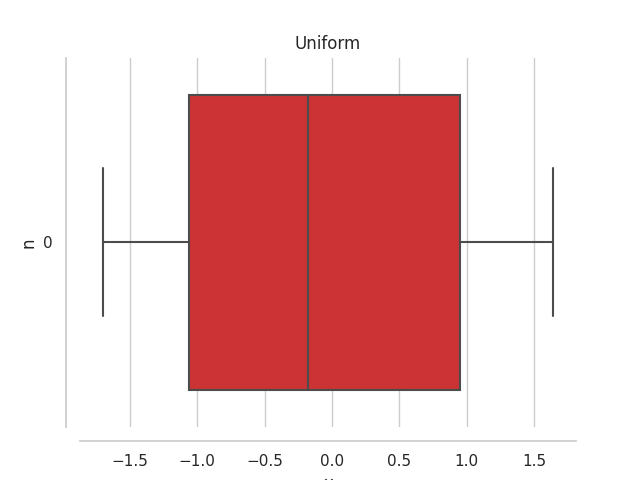
\includegraphics[scale=0.8]{Uniform100.png}
    \caption{Равномерное распределение с размером выборки 100}
    \label{fig:normal}
\end{figure}

\subsection{Доля выбросов}
\begin{table}[H]
	\centering
	\begin{tabular}{|l|c|c|}
		\hline
		Выборка & Доля выбросов	& $P^T_B$\\\hline
		\hline
		Нормальное n = 20 & 0.0229 & 0.007\\\hline
		Нормальное n = 100 & 0.0096 & 0.007\\\hline
		Коши n = 20 & 0.1526 & 0.156\\\hline
		Коши n = 100 & 0.1555 & 0.156\\\hline
		Лапласа n = 20 & 0.0744 & 0.063\\\hline
		Лапласа n = 100 & 0.0663 & 0.063\\\hline
		Пуассона n = 20 & 0.0238 & 0.008\\\hline
		Пуассона n = 100 & 0.0096 & 0.008\\\hline
		Равномерное n = 20 & 0.0027 & 0\\\hline
		Равномерное n = 100 & 0 & 0\\\hline
	\end{tabular}
	\caption{Практическая доля выбросов}
\end{table}

\begin{table}[H]
	\centering
	\begin{tabular}{|l|c|c|c|c|c|}
		\hline
		Распределение & $Q_1^T$	& $Q_3^T$ & $X_1^T$ & $X_2^T$ & $P_B^T$\\\hline
		\hline
		Нормальное & -0.674 & 0.674 & -2.698 &  2.698 & 0.007\\\hline
		Коши & -1 & 1 & -4 & 4 & 0.156\\\hline
		Лапласа & -0.490 & 0.490 & -1.961 & 1.961 & 0.063\\\hline
		Пуассона & 8 & 12 & 2 & 18 & 0.008\\\hline
		Равномерное & -0.866 & 0.866 & -3.464 & 3.464 & 0\\\hline
	\end{tabular}
	\caption{Теоретическая вероятность выбросов}
\end{table}

\section{Обсуждение}
Боксплот Тьюки позволяет удобно продемонстрировать характеристики заданного распределения: медиану, первый и третий квартили, выбросы, максимальные и минимальные значения. Анализировать такой график проще и удобнее, чем аналитические расчёты.

Таблицы показывают, что для всех распределений чем больше размерность выборки, тем ближе найденная доля выбросов к теоретической оценке. В распределении Коши доля выбросов значительно выше, чем во всех остальных распределениях, а у равномерного выбросы почти не наблюдаются.
\end{document}